% Figure from MATH 556 notes, section 39 (closed and non-closed graphs). Added, not from lecture.
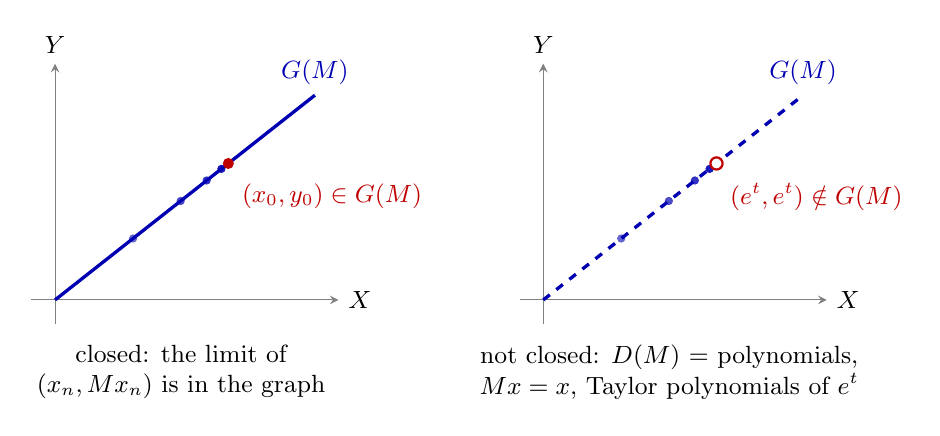
\begin{tikzpicture}[>=stealth, font=\small]
  \begin{scope}
    \draw[->, gray] (-0.3,0) -- (3.6,0) node[right, text=black] {$X$};
    \draw[->, gray] (0,-0.3) -- (0,3.0) node[above, text=black] {$Y$};
    \draw[very thick, blue!70!black] (0,0) -- (3.3,2.6) node[above, font=\small] {$G(M)$};
    \foreach \t/\o in {0.9/60,1.45/70,1.75/80,1.92/90} { \fill[blue!70!black, opacity=0.\o] ({\t*1.1},{\t*0.8667}) circle (1.5pt); }
    \fill[red!75!black] (2.2,1.733) circle (2pt);
    \node[red!75!black, anchor=north west, align=left] at (2.25,1.6) {$(x_0, y_0) \in G(M)$};
    \node[anchor=north, align=center] at (1.6,-0.45) {closed: the limit of\\ $(x_n, Mx_n)$ is in the graph};
  \end{scope}
  \begin{scope}[xshift=6.2cm]
    \draw[->, gray] (-0.3,0) -- (3.6,0) node[right, text=black] {$X$};
    \draw[->, gray] (0,-0.3) -- (0,3.0) node[above, text=black] {$Y$};
    \draw[very thick, blue!70!black, dashed] (0,0) -- (3.3,2.6) node[above, font=\small] {$G(M)$};
    \foreach \t/\o in {0.9/60,1.45/70,1.75/80,1.92/90} { \fill[blue!70!black, opacity=0.\o] ({\t*1.1},{\t*0.8667}) circle (1.5pt); }
    \draw[red!75!black, thick, fill=white] (2.2,1.733) circle (2.2pt);
    \node[red!75!black, anchor=north west, align=left] at (2.25,1.6) {$(e^t, e^t) \notin G(M)$};
    \node[anchor=north, align=center] at (1.6,-0.45) {not closed: $D(M)$ = polynomials,\\ $Mx = x$, Taylor polynomials of $e^t$};
  \end{scope}
\end{tikzpicture}
